\documentclass{article}
%\usepackage[english]{babel}%
\usepackage{graphicx}
\usepackage{tabulary}
\usepackage{tabularx}
\usepackage[table,xcdraw]{xcolor}
\usepackage{pdflscape}
%\usepackage{gensymb}
\usepackage{lastpage}
\usepackage{multirow}
\usepackage{xcolor}
\usepackage{cancel}
\usepackage{amsmath}
\usepackage[table]{xcolor}
\usepackage{fixltx2e}
\usepackage[T1]{fontenc}
\usepackage[utf8]{inputenc}
\usepackage{ifthen}
\usepackage{fancyhdr}
\usepackage[utf8]{inputenc}
\usepackage{tikz}
\usepackage[document]{ragged2e}
\usepackage[margin=1in,top=1.2in,headheight=57pt,headsep=0.1in]
{geometry}
\usepackage{ifthen}
\usepackage{fancyhdr}
\everymath{\displaystyle}
\usepackage[document]{ragged2e}
\usepackage{fancyhdr}
\usepackage{mathabx}
\usepackage{textcomp,mathcomp}
\usepackage[shortlabels]{enumitem}
\everymath{\displaystyle}
\linespread{2}%controls the spacing between lines. Bigger fractions means crowded lines%
\linespread{1.3}%controls the spacing between lines. Bigger fractions means crowded lines%
\pagestyle{fancy}
\setlength{\headheight}{56.2pt}
\usepackage{soul}
\usepackage{siunitx}

%\usepackage{textcomp}
\usetikzlibrary{shapes.multipart, shapes.geometric, arrows}
\usetikzlibrary{calc, decorations.markings}
\usetikzlibrary{arrows.meta}
\usetikzlibrary{shapes,snakes}
\usetikzlibrary{quotes,angles, positioning}
%\chead{\ifthenelse{\value{page}=1}{
\includegraphics[scale=0.3]{BassettCTCLogo}}}
%\rhead{\ifthenelse{\value{page}=1}{Final Exam}{}}
%\lhead{\ifthenelse{\value{page}=1}{Water Treatment - Oct-Dec 2022}{\textbf Final Exam}}
%\rfoot{\ifthenelse{\value{page}=1}{}{}}
%
%\cfoot{}
%\lfoot{Page \thepage\ of \pageref{LastPage}}
%\renewcommand{\headrulewidth}{2pt}
%\renewcommand{\footrulewidth}{1pt}
\graphicspath{ {./images/} }
\begin{document}
\begin{enumerate}

\item A reservoir is 40 feet tall. Find the pressure at the bottom of the reservoir.

$40 \mathrm{ft} \times 0.433 \mathrm{psi} / \mathrm{ft}=17.3 \mathrm{psi}$

\vspace{0.4cm}

\item Find the height of water in a tank if the pressure at the bottom of the tank is 12 psi.

$12 \mathrm{psi} \div 0.433 \mathrm{psi} / \mathrm{ft}=27.7 \mathrm{ft}$

\vspace{0.4cm}

\item If a pump discharge pressure gauge read 10 psi, the height of the water corresponding to this pressure would be:
$$10 \enspace psi \times \dfrac{2.31 \enspace ft}{psi}=23.1 \enspace ft$$\\
\vspace{0.4cm}
\item A water tank is filled to depth of 22 feet. What is the psi at the bottom of the tank?\\
 \vspace{0.2cm}
Solution:\\ 
 \vspace{0.2cm}
$
22 \enspace \cancel{ft}*\dfrac{0.433psi}{\cancel{ft \enspace head}}=\boxed{9.5 \text { psi }}
$
  \vspace{0.2cm}
\item The static pressure in a water main is 85 psi. What elevation of water is needed to provide that kind of pressure?\\
 \vspace{0.2cm}
Solution:\\ 
 \vspace{0.2cm}
$
85 \enspace \cancel{psi}*\dfrac{ft \enspace head}{0.433\cancel{psi}}=\boxed{196.3 \text { feet }}
$
 
 \vspace{0.2cm}

\item The pressure at the top of the hill is 62 psi. The pressure at the bottom of the hill, 60 feet below, is 100 psi. The water is flowing uphill at 120 gpm. What is the friction loss, in feet, in the pipe?\\
\vspace{0.2cm}
\begin{tikzpicture}[scale=2]
\draw[ultra thick,-](0.8,0.8) -- (1,0.8)node [at start, below,  black]{\small{}} node [anchor=north west, black]{} node [at start, left, black] (n){};;
\draw[ultra thick,-](-1,0) -- (-0.2,0)node [at start, below,  black]{\small{}} node [anchor=north west, black]{} node [at start, left, black] (n){};;
\draw[ultra thick,-](-0.2,0) -- (0.8,0.8)node [at start, below,  black]{\small{}} node [anchor=north west, black]{} node [at start, left, black] (n){};;
\draw [<->] (1,0) -- (1,0.78) node [midway, midway] {\hspace{1.5cm}60'};
 \node at (-0.5,0.11) {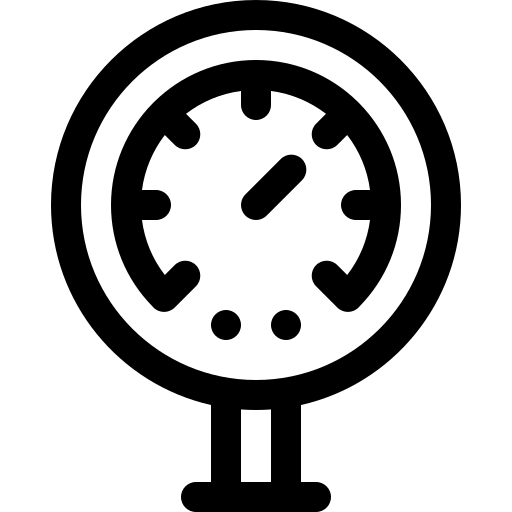
\includegraphics[width=0.5cm]{PressureGuageIcon.png}};
  \node at (1,0.91) {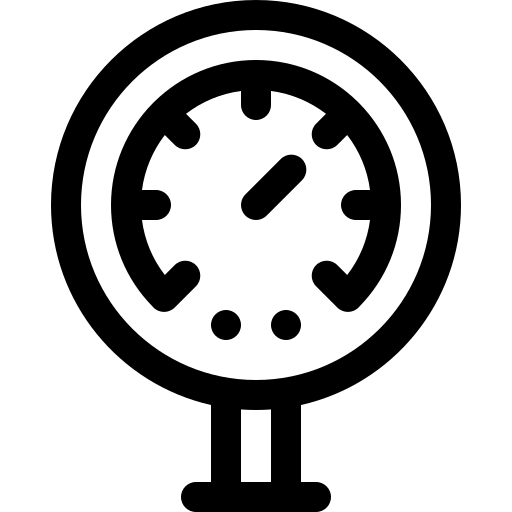
\includegraphics[width=0.5cm]{PressureGuageIcon.png}};

\draw (0,0) .. controls (0.98,1.05) and (1.02,1.05) .. (2,0);
\draw (1.1,1.05) node[anchor=north west] {$Pressure=62psi$};
\draw (-0.65,0.5) node[anchor=north east] {$Flow=120 gpm$};
\draw (-0.65,0.3) node[anchor=north east] {$Pressure=100psi$};
\end{tikzpicture}\\
\vspace{0.2cm}
Total headloss = Headloss due to elevation gain + Headloss due to friction\\
\vspace{0.2cm}
$\implies$ Headloss due to friction = Total headloss - Headloss due to elevation gain\\
\vspace{0.2cm}
Total headloss = $(100 - 62)\enspace \cancel{psi}* \dfrac{ft \enspace head}{0.433\cancel{psi}}=87.8 ft $\\
Headloss due to elevation gain = $60 \enspace ft $\\
$\implies$ Headloss due to friction = $87.8-60=\boxed{27.8 \enspace ft}$\\
\vspace{0.2cm}
 \item Find the force on a 12-inch valve if the water pressure within the line is 60 psi. Express your answer in tons.

$\textrm{Force}= \textrm{Pressure} \times \textrm{Area}$\\
\vspace{0.3cm}
$\implies 60 \enspace \dfrac{\mathrm{lbs}}{\mathrm{in^2}}*0.785 *(12 \mathrm{in})^2*\dfrac{1 \mathrm{ton}}{2000 \mathrm{lbs}} =\boxed{3.39 \enspace\mathrm{tons}}$
\vspace{0.3cm}

\item A water tank is 15 feet deep and 30 feet in diameter. What is the force exerted on a 6-inch valve at the bottom of the tank?\\
\vspace{0.5cm}
$\textrm{Force}= \textrm{Pressure} \times \textrm{Area}$\\
\vspace{0.5cm}
$\implies 15 \enspace\mathrm{ft}* \dfrac{0.433 \enspace \mathrm{psi}}{\mathrm{ft}}*0.785 *(6 \mathrm{in})^2 =\boxed{183 \enspace\mathrm{lbs}}$\\


\item The efficiency of a well pump is determined to be $75 \%$. The efficiency of the motor is estimated at $94 \%$. What is the efficiency of the well?\\
 \vspace{0.2cm}
Solution:\\ 
 \vspace{0.2cm}
$Well \enspace efficiency=\eta_m * \eta_p \implies 0.94 \times 0.75=0.705 \times 100=\boxed{71 \%}$
 \vspace{0.2cm}

  \item Water is being pumped from a reservoir to a storage tank on a hill. The elevation difference between water levels is 1200 feet. Find the pump size (in Hp) required to fill the tank at a rate of 120 gpm.\\
  \vspace{0.2cm}
\begin{tikzpicture}[scale=1]
\draw (0,0) .. controls (1.98,3.5) and (2.02,3.5) .. (4,0);
\node[cylinder, 
    draw = violet, 
    text = purple,
    cylinder uses custom fill, 
    cylinder body fill = blue!10, 
    cylinder end fill = magenta!40,
    aspect = 0.1, 
    shape border rotate = 90] (c) at (2,3.0) {Storage};
\node[cylinder, 
    draw = violet, 
    text = purple,
    cylinder uses custom fill, 
    %cylinder body fill = magenta!10, 
    %cylinder end fill = magenta!40,
    minimum size = 0.3cm, aspect = 0.1,
    shape border rotate = 90] (c) at (2,3.5) {\hspace{0.25cm}{Water}\hspace{0.25cm}};

  \node at (-3,0.1) {\includegraphics[width=3cm]{PumpIcon.png}};
   \node at (-3,-0.8) {
\includegraphics[width=2cm]{WaterReservoirIcon.png}};
   
\draw [ultra thick, -] (-3,-.9) -- (-3,0) node [midway, below] {};
\draw [ultra thick, -] (-3.28,0.63) -- (-3.28,3.1) node [midway, below] {};
\draw [ultra thick, ->] (-3.28,3.1) -- (1.2,3.1) node [midway, below] {};
\draw [ultra thick, ->] (-3.28,3.1) -- (1.2,3.1) node [midway, below] {};
\draw[dashed] (-1.8,-1) -- (2.5,-1);
\draw [<->] (2,-1) -- (2,3.25) node [midway, below] {\hspace{5cm}Elevation difference = 1200 ft};
\draw (0.5,3.7) node[anchor=north east] {$Flow = 120 gpm$};
\end{tikzpicture}\\
\vspace{0.2cm}
Solution:\\
\vspace{0.2cm}
water Hp = flow * head\\
$120GPM*1,200ft*\dfrac{Hp}{3,960 GPM-ft}=\boxed{Water \enspace Hp = 36.4Hp}$\\
\item If a pump is operating at 2,200 gpm and 60 feet of head, what is the water horsepower? If the pump efficiency is 71\%, what is the brake horsepower?\\
\vspace{0.2cm}
Solution:\\
\vspace{0.2cm}
water Hp = flow * head\\
$2,200GPM*60ft*\dfrac{Hp}{3,960 GPM-ft}=\boxed{Water \enspace Hp = 33.3Hp}$\\
\vspace{0.4cm}
pump Hp = brake Hp * pump efficiency\\
$brake \enspace Hp = \dfrac{33.3}{0.71}=\boxed{Brake \enspace Hp=47Hp}$
 \vspace{0.2cm}


\end{enumerate}
\end{document}